\documentclass[10pt, a5paper]{article}
\usepackage{pdfpages}
\usepackage{parallel}
\usepackage[T2A]{fontenc}
\usepackage{ucs}
\usepackage[utf8x]{inputenc}
\usepackage[polish,english,russian]{babel}
\usepackage{hyperref}
\usepackage{rotating}
\usepackage[inner=2cm,top=1.8cm,outer=2cm,bottom=2.3cm,nohead]{geometry}
\usepackage{listings}
\usepackage{graphicx}
\usepackage{wrapfig}
\usepackage{longtable}
\usepackage{indentfirst}
\usepackage{array}
\newcolumntype{P}[1]{>{\raggedright\arraybackslash}p{#1}}
\frenchspacing
\usepackage{fixltx2e} %text sub- and superscripts
\usepackage{icomma} % коскі ў матэматычным рэжыме
\PreloadUnicodePage{4}

\newcommand{\longpage}{\enlargethispage{\baselineskip}}
\newcommand{\shortpage}{\enlargethispage{-\baselineskip}}

\def\switchlang#1{\expandafter\csname switchlang#1\endcsname}
\def\switchlangbe{
\let\saverefname=\refname%
\def\refname{Літаратура}%
\def\figurename{Іл.}%
}
\def\switchlangen{
\let\saverefname=\refname%
\def\refname{References}%
\def\figurename{Fig.}%
}
\def\switchlangru{
\let\saverefname=\refname%
\let\savefigurename=\figurename%
\def\refname{Литература}%
\def\figurename{Рис.}%
}

\hyphenation{admi-ni-stra-tive}
\hyphenation{ex-pe-ri-ence}
\hyphenation{fle-xi-bi-li-ty}
\hyphenation{Py-thon}
\hyphenation{ma-the-ma-ti-cal}
\hyphenation{re-ported}
\hyphenation{imp-le-menta-tions}
\hyphenation{pro-vides}
\hyphenation{en-gi-neering}
\hyphenation{com-pa-ti-bi-li-ty}
\hyphenation{im-pos-sible}
\hyphenation{desk-top}
\hyphenation{elec-tro-nic}
\hyphenation{com-pa-ny}
\hyphenation{de-ve-lop-ment}
\hyphenation{de-ve-loping}
\hyphenation{de-ve-lop}
\hyphenation{da-ta-ba-se}
\hyphenation{plat-forms}
\hyphenation{or-ga-ni-za-tion}
\hyphenation{pro-gramming}
\hyphenation{in-stru-ments}
\hyphenation{Li-nux}
\hyphenation{sour-ce}
\hyphenation{en-vi-ron-ment}
\hyphenation{Te-le-pathy}
\hyphenation{Li-nux-ov-ka}
\hyphenation{Open-BSD}
\hyphenation{Free-BSD}
\hyphenation{men-ti-on-ed}
\hyphenation{app-li-ca-tion}

\def\progref!#1!{\texttt{#1}}
\renewcommand{\arraystretch}{2} %Іначай формулы ў матрыцы зліпаюцца з лініямі
\usepackage{array}

\def\interview #1 (#2), #3, #4, #5\par{

\section[#1, #3, #4]{#1 -- #3, #4}
\def\qname{LVEE}
\def\aname{#1}
\def\q ##1\par{{\noindent \bf \qname: ##1 }\par}
\def\a{{\noindent \bf \aname: } \def\qname{L}\def\aname{#2}}
}

\def\interview* #1 (#2), #3, #4, #5\par{

\section*{#1\\{\small\rm #3, #4. #5}}

\def\qname{LVEE}
\def\aname{#1}
\def\q ##1\par{{\noindent \bf \qname: ##1 }\par}
\def\a{{\noindent \bf \aname: } \def\qname{L}\def\aname{#2}}
}


\begin{document}

\title{<<Покращення вже сьогодні>> или оптимизация процесса разработки}%\footnote{Текст данных и последующих тезисов, кроме специально оговоренных случаев, доступен под лицензией Creative Commons Attribution-ShareAlike 3.0}

\author{Николай Маржан, Александр Лутай\footnote{Киев, Украина; \url{delgod@delgod.com}}}
\maketitle

\begin{abstract}
The paper describes organizational transformations at the company that resulted into the improved actual efficiency of the developers due to lower bureaucratic burden and related time losses, expenses associated with the setup of development environment, costs associated with waiting for QA/user’s feedback, and manual testing costs. Special attention is payed to involved open source instruments.
\end{abstract}

По мере роста IT"=компании, разработчики в ней начинают все меньше  заниматься непосредственно написанием кода и все больше "--- сопутствующими задачами: заполнением метрик в системе трекинга ошибок, написанием огромного количества писем для того, чтобы договориться с разработчиками другого компонента, ожиданием ответов со стороны заказчика/QA/потребителя, развертыванием среды разработки, ручным тестированием и т.~д. С увеличением кодовой базы и накоплением взаимосвязей компонентов в продукте все труднее предсказать дату выхода новой версии. Подход с выпуском новых версий продукта <<по готовности>> всегда срывает все объявленые заказчику сроки, даже самые пессимистичные.

Ниже рассмотрен комплекс мер, направленных на увеличение эффективности разработки и снижение ее бюрократизации, примененный в компании PortaOne, Inc. и приведший к существенной оптимизации организационных процессов.

Практически все разработчики ПО "--- люди, которые любят писать новый код и не любят тратить время на сопутствующие этому процессу издержки.

Чтобы сделать разработчиков счастливыми, были предприняты следующие шаги:

\begin{itemize}
  \item отменена заморозка веток в системе контроля версий;
  \item экстремально сокращено время необходимое на развертывание среды разработки;
  \item организован автоматический запуск юнит"=тестов на каждый коммит;
  \item организован автоматический запуск тяжелых функциональных тестов;
  \item ускоренно получение отзывов (багрепортов) от отдела QA и заказчика.
\end{itemize}

Целью заказчика разработки (внешнего или внутреннего) является получение новых функциональных возможностей (<<фич>>) как можно быстрее, при стабильно низком количестве программных ошибок (багов).

Чтобы сделать заказчика счастливым, были предприняты следующие шаги:

\begin{itemize}
  \item организован выход новых версий продукта, с заказанными новыми функциональными возможностями, точно в срок, по календарю;
  \item т.~к. новые функциональные возможности могут быть реализованы с ошибками, организован выпуск новых версий продукта только с исправлениями (без новых функциональных возможностей) точно в срок, по календарю;
  \item чтобы уменьшить количество ошибок, все изменения перед внесением в центральный репозиторий проходят процедуру рецензирования и автоматически проверяются тестами.
\end{itemize}

\subsection*{Отмена заморозки веток в системе контроля версий}

Для того, чтобы отдел QA мог уменьшить количество ошибок и обеспечить стабильность, перед выпуском новой версии продукта нужно временно ограничивать количество вносимых изменений.

Назовем запрет на добавление новой функциональности "--- желтой зоной. А запрет на любые изменения "--- красной. Логическим завершением красной зоны является выход новой версии продукта.

Такой подход создает искусственные временные издержки на фиксацию (коммит)  готовых изменений в репозитории. Разработчик, который написал новый код, не может зафиксировать изменения, в результате он должен не забывать о них довольно продолжительный период времени. Когда разработчиков много, количество зависших коммитов может увеличиваться до нескольких сотен.

Чтобы не рассеивать внимание разработчиков и дать возможность коммитить в любой момент времени любую функциональность, подход был изменен следующим образом:

\begin{figure}
  \centering
  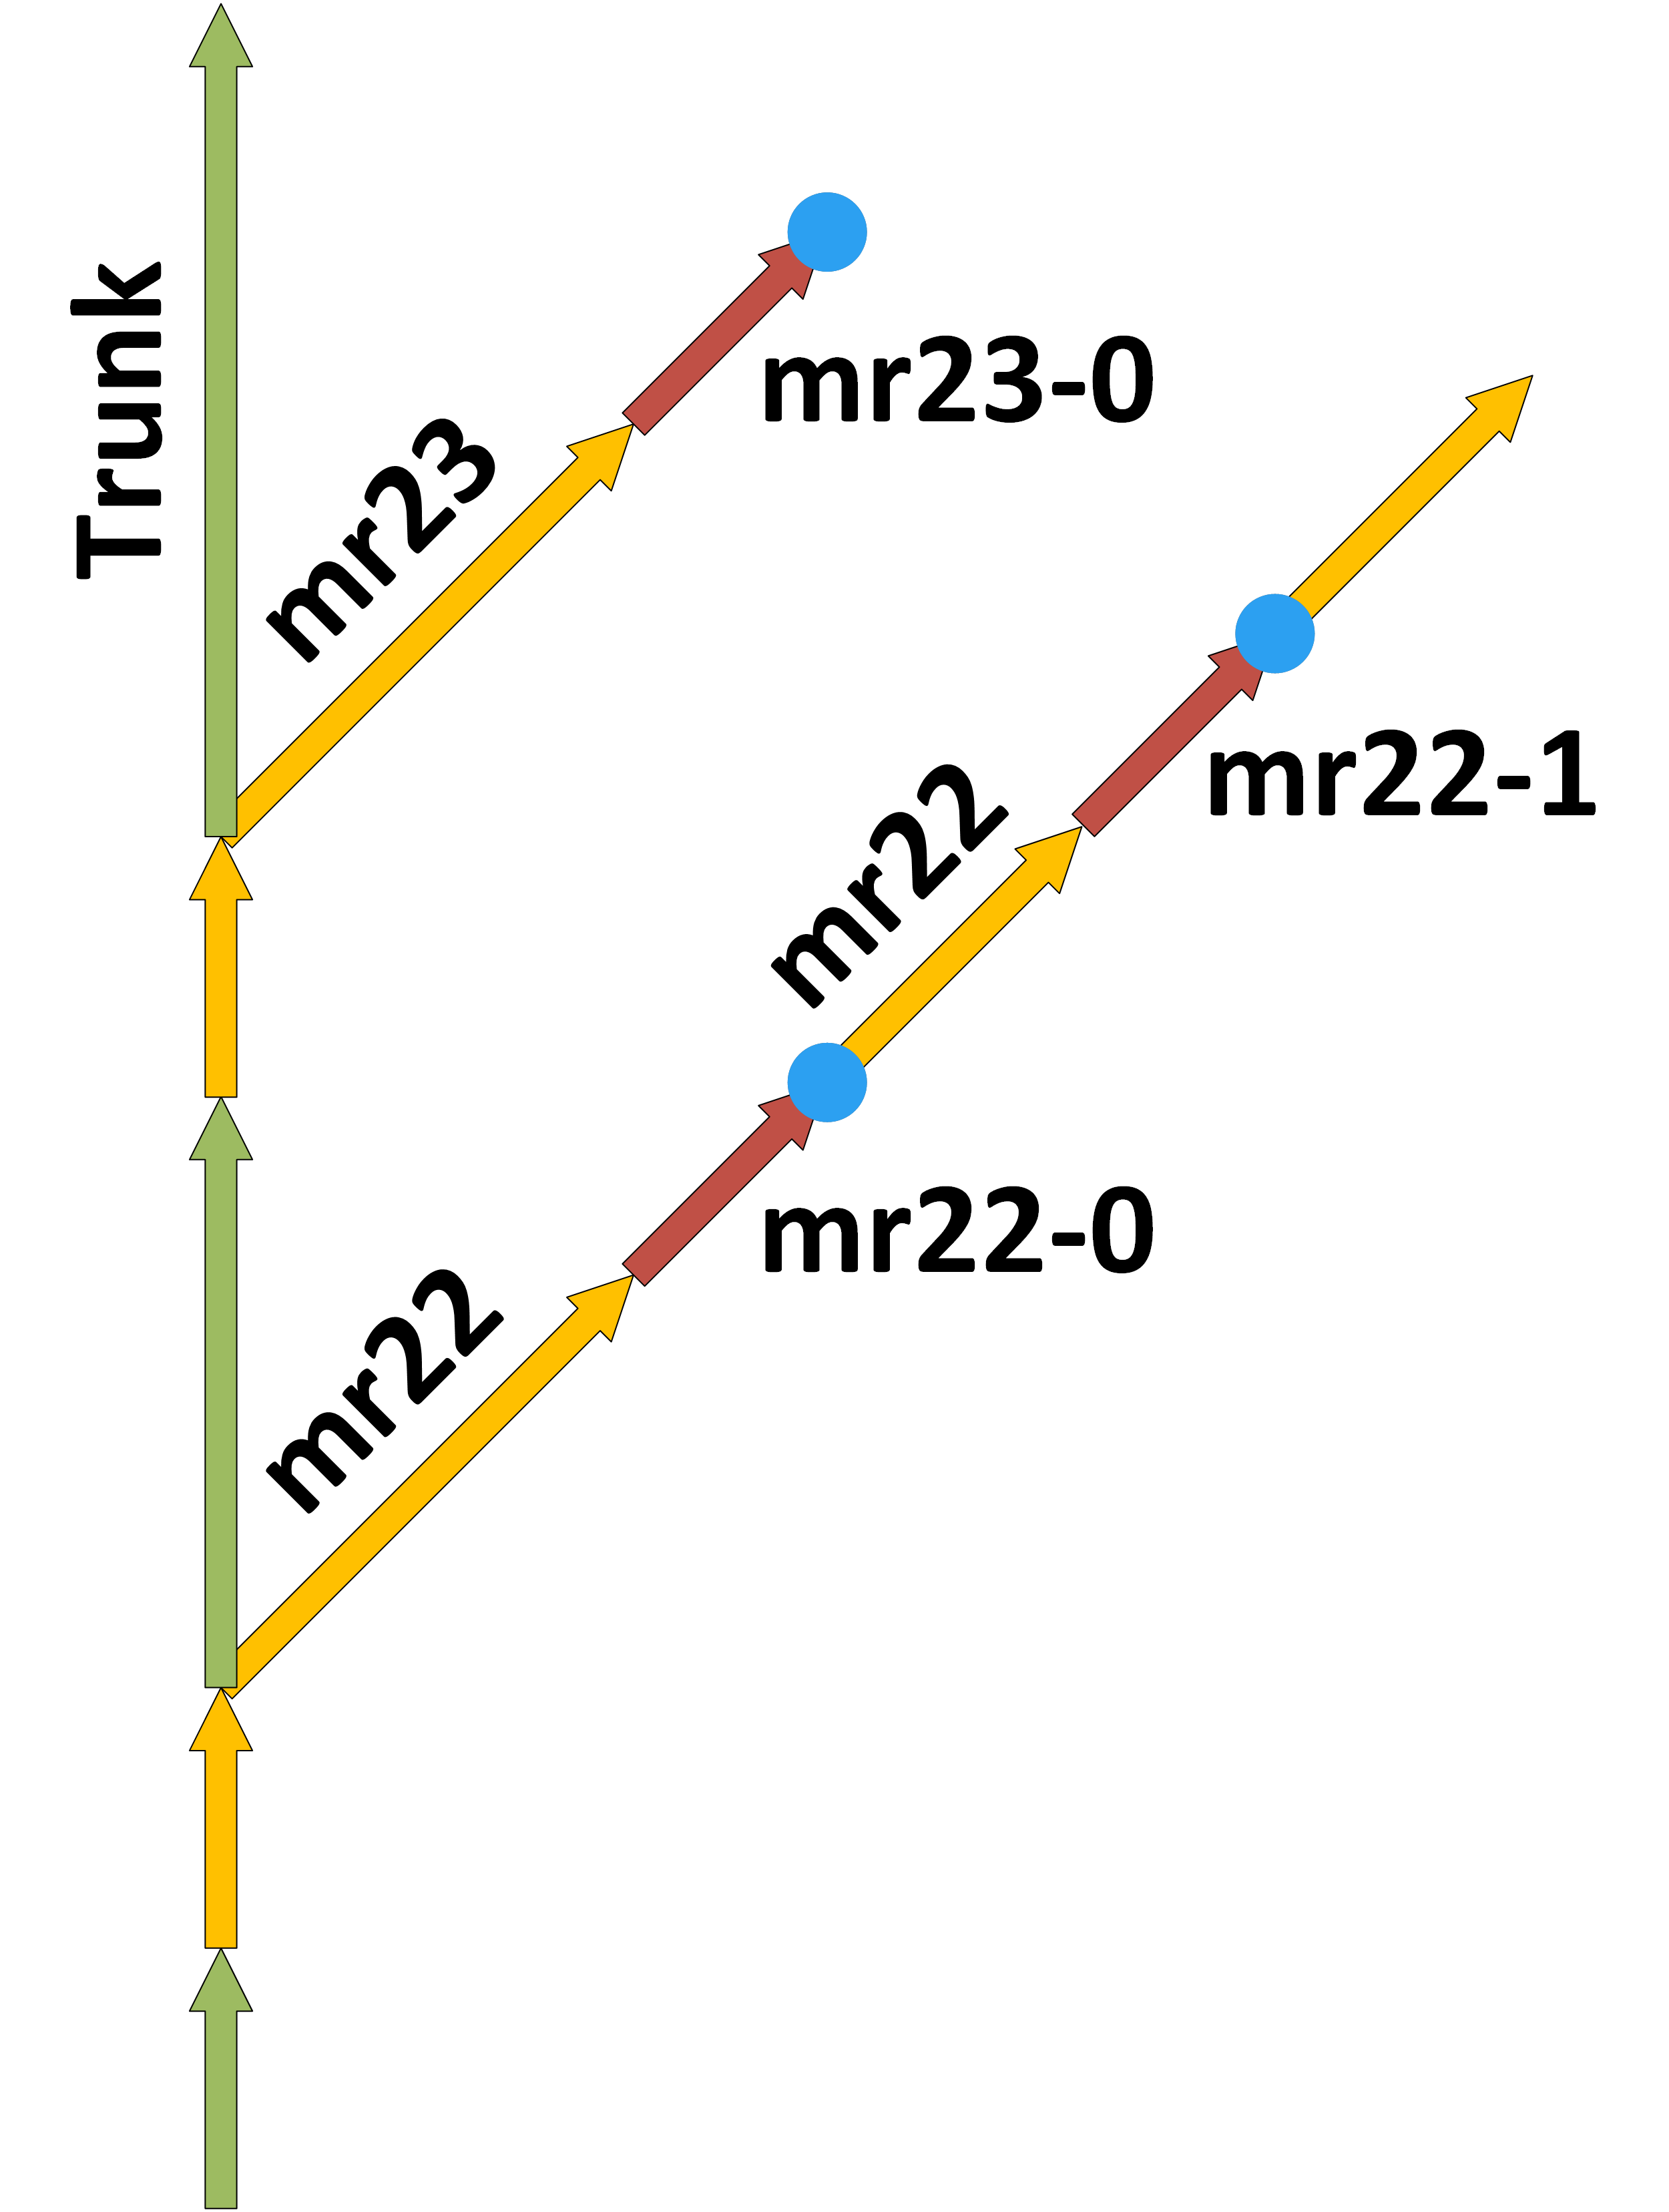
\includegraphics[height=5.5cm]{05_zones_old.png}
\end{figure}



\begin{figure}
  \centering
  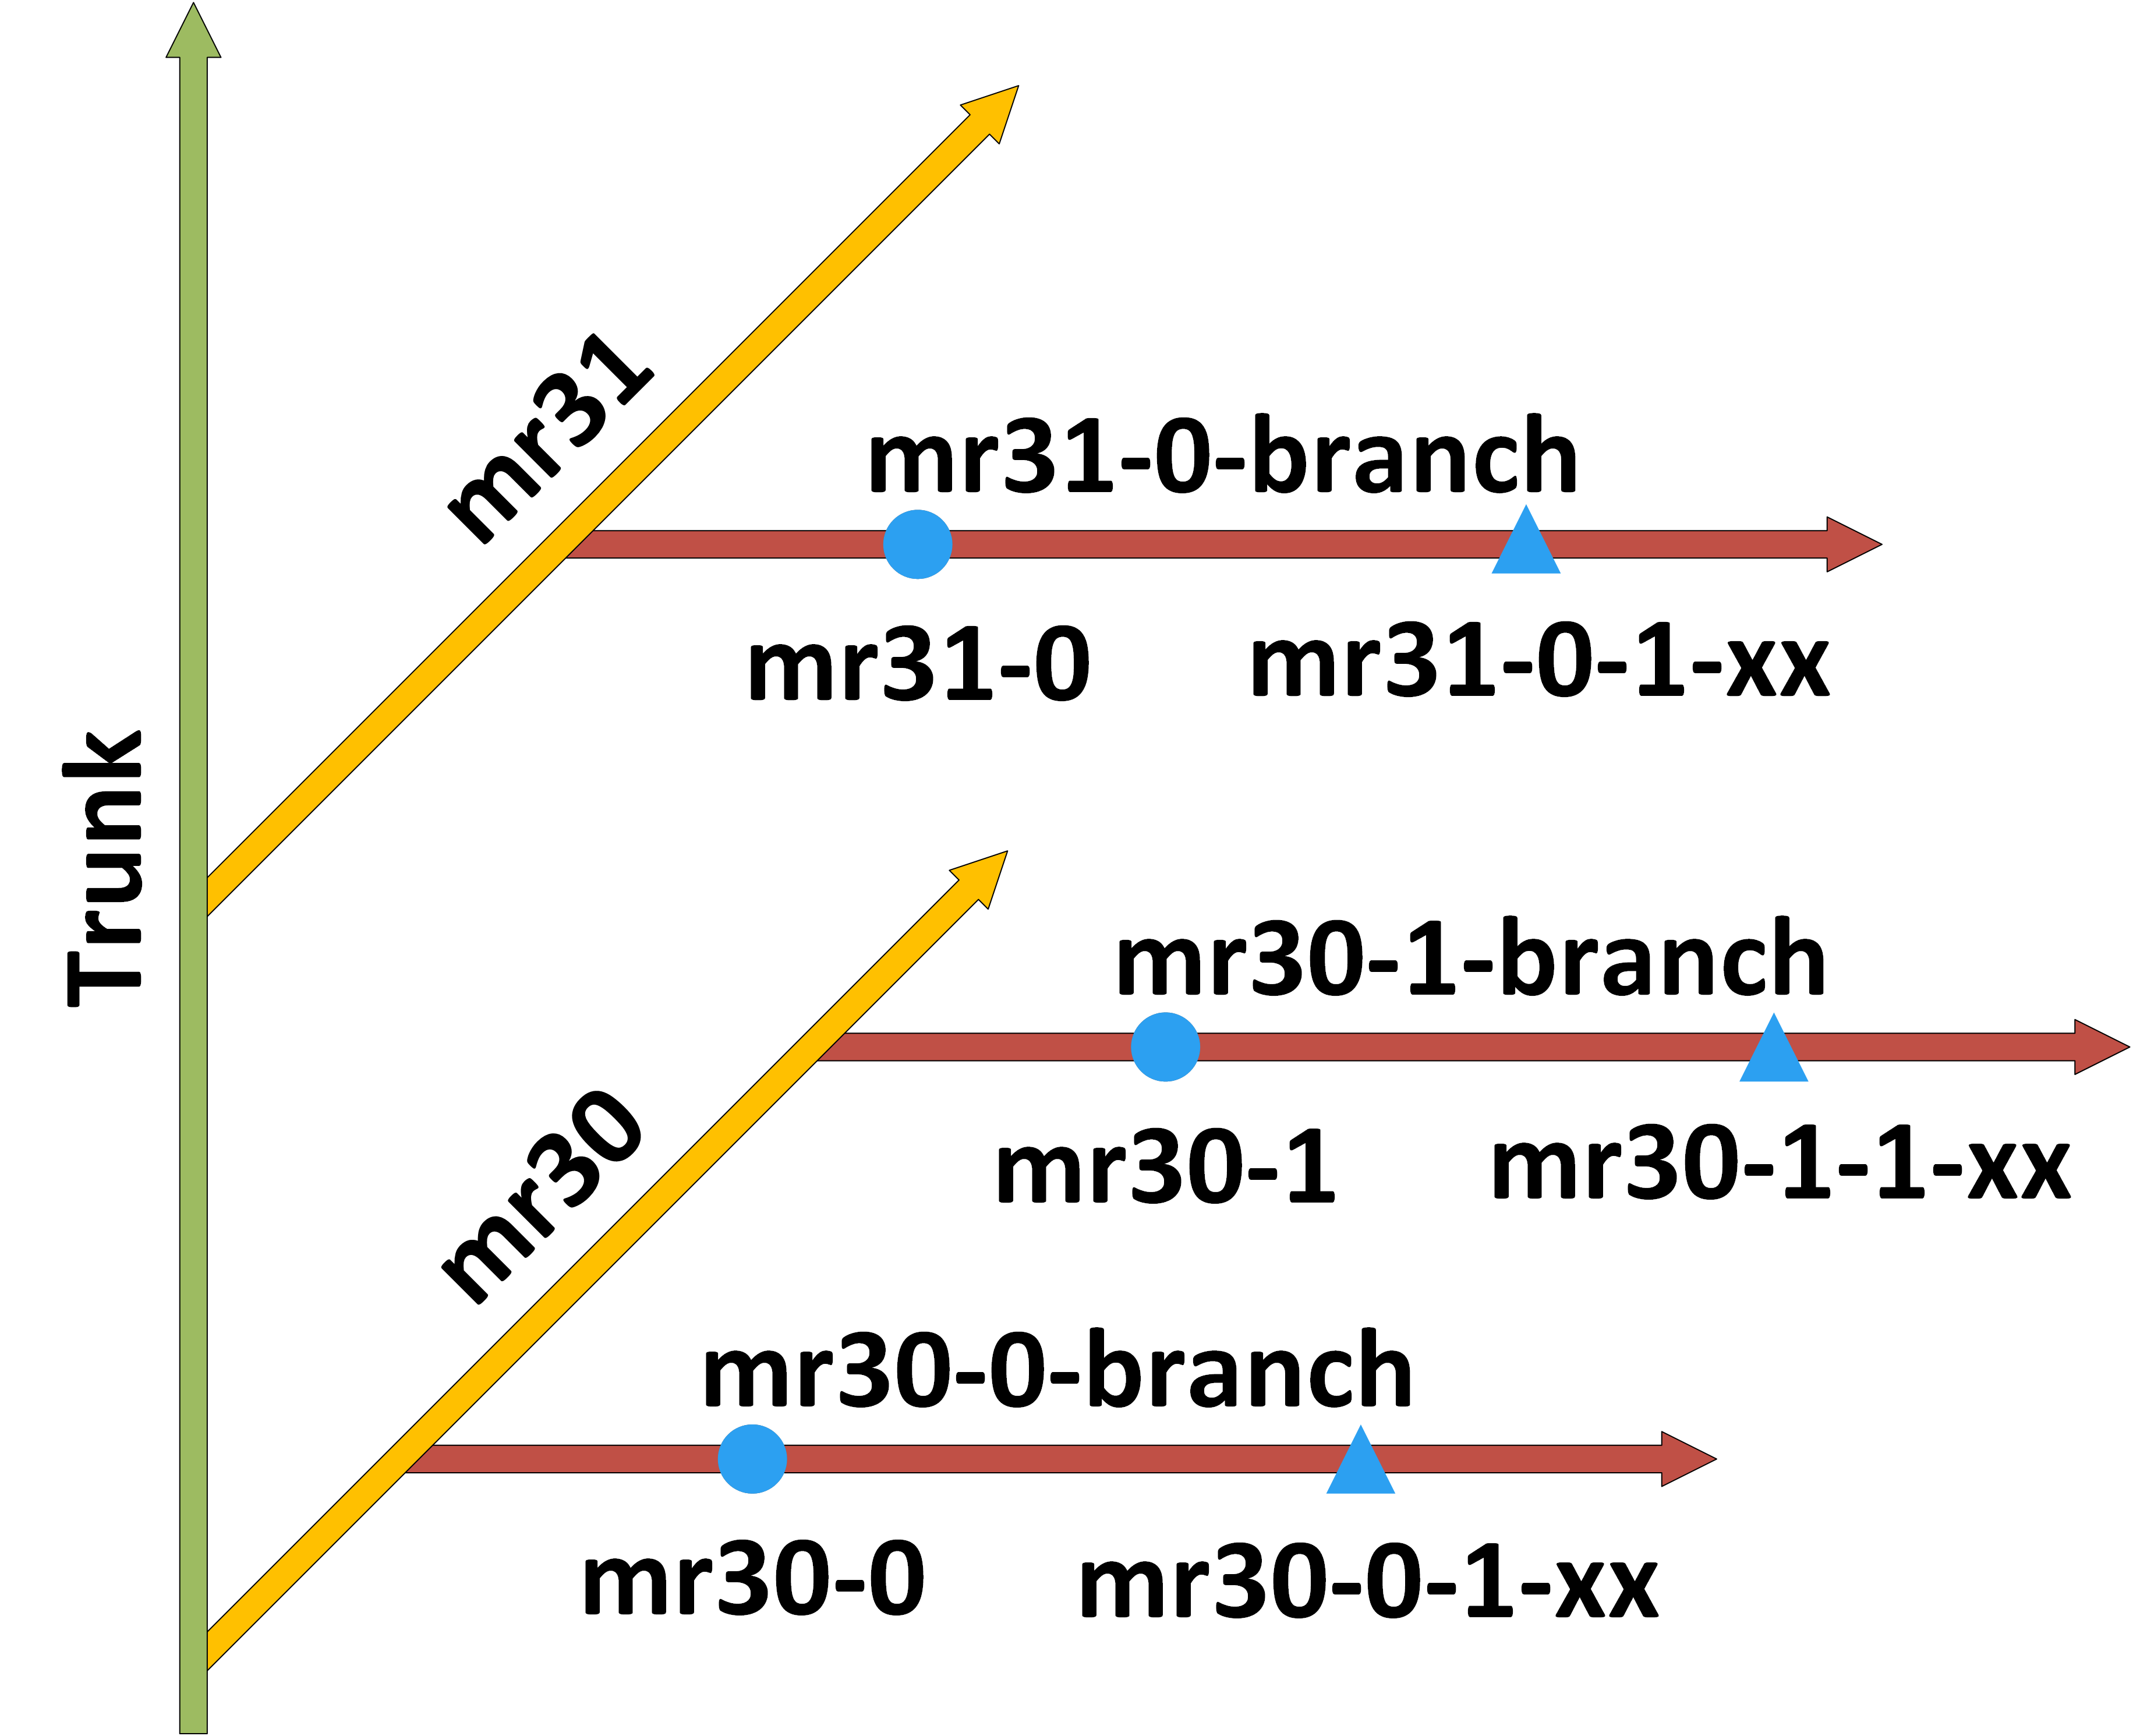
\includegraphics[width=6cm]{05_zones.png}
\end{figure}

Главная ветвь разработки (trunk/master) всегда открыта для приема любых новых функциональных возможностей.

В определенный момент времени (по календарю) от главной ветви <<отщепляется>> новая ветвь, в которой будет проходить стабилизация готовых на тот момент программных возможностей. Эта ветвь сразу становится желтой, т.~е. в неё запрещено добавлять новые возможности, только стабилизировать текущие.

В определенный момент времени от желтой ветви отщепляется красная ветвь. В красную ветвь можно коммитить только по запросу QA отдела.
В определенный момент времени (по календарю), на красной ветви проставляется аннотированная метка (тег) нового релиза.
К этому моменту отдел QA должен завершить тестирование новой версии продукта. Если какие"=то новые программные возможности не готовы и блокируют выпуск новой версии, они должны быть удалены.

Если после проставления аннотированной метки, заказчик или отдел поддержки/эксплуатации находит критический баг, тогда отдел QA запрашивает коммит с исправлением в красную ветвь. После этого на красной ветви проставляется аннотированная метка хотфикса.
Данный подход позволяет разработчикам фиксировать изменения в любой момент времени, потому что главная ветка проекта всегда готова к приему любых изменений, желтые ветки в любой момент готовы к приему исправлений.

\subsection*{Наращивание новых функций и стабильность}

Есть два типа заказчиков: первые хотят стабильности, вторые заказывают новые функциональные возможности и стремятся ими воспользоваться как можно раньше.

Для первого типа заказчиков предлагается раз в год выпускать long-term support (LTS) релиз (релиз "--- это нулевой билд, x.0 версия), который будет стабилизироваться в течении года выпуском 6 билдов (версии x.1, x.2 и т.д.) только с исправлениями.
Для второго типа заказчиков предлагается переходить на обычные релизы по мере их выхода. Зачастую в очень сложных проектах новые программные возможности не всегда удовлетворяют заказчика с первого раза. Потому, чаще всего, после сдачи новых возможностей, заказчику нужно немного исправить поведение продукта. Поэтому для каждого обычного релиза выпускается один стабилизационный билд.
Заказчику нужно некоторое время для запуска новой версии продукта в промышленное использование, потому после выхода нового релиза команда разработчиков сразу приступает к выпуску стабилизационного билда к предыдущему релизу. Одновременно с этим разработчики бэкпортируют все правки в LTS релиз и выпускают стабилизационный билд для LTS тоже. Т.~о. разработчики не ждут отзыва заказчиков, для которых был выпущен новый релиз, а исправляют предыдущий, на который к этому моменту собраны жалобы.

~

\begin{figure}
  \centering
  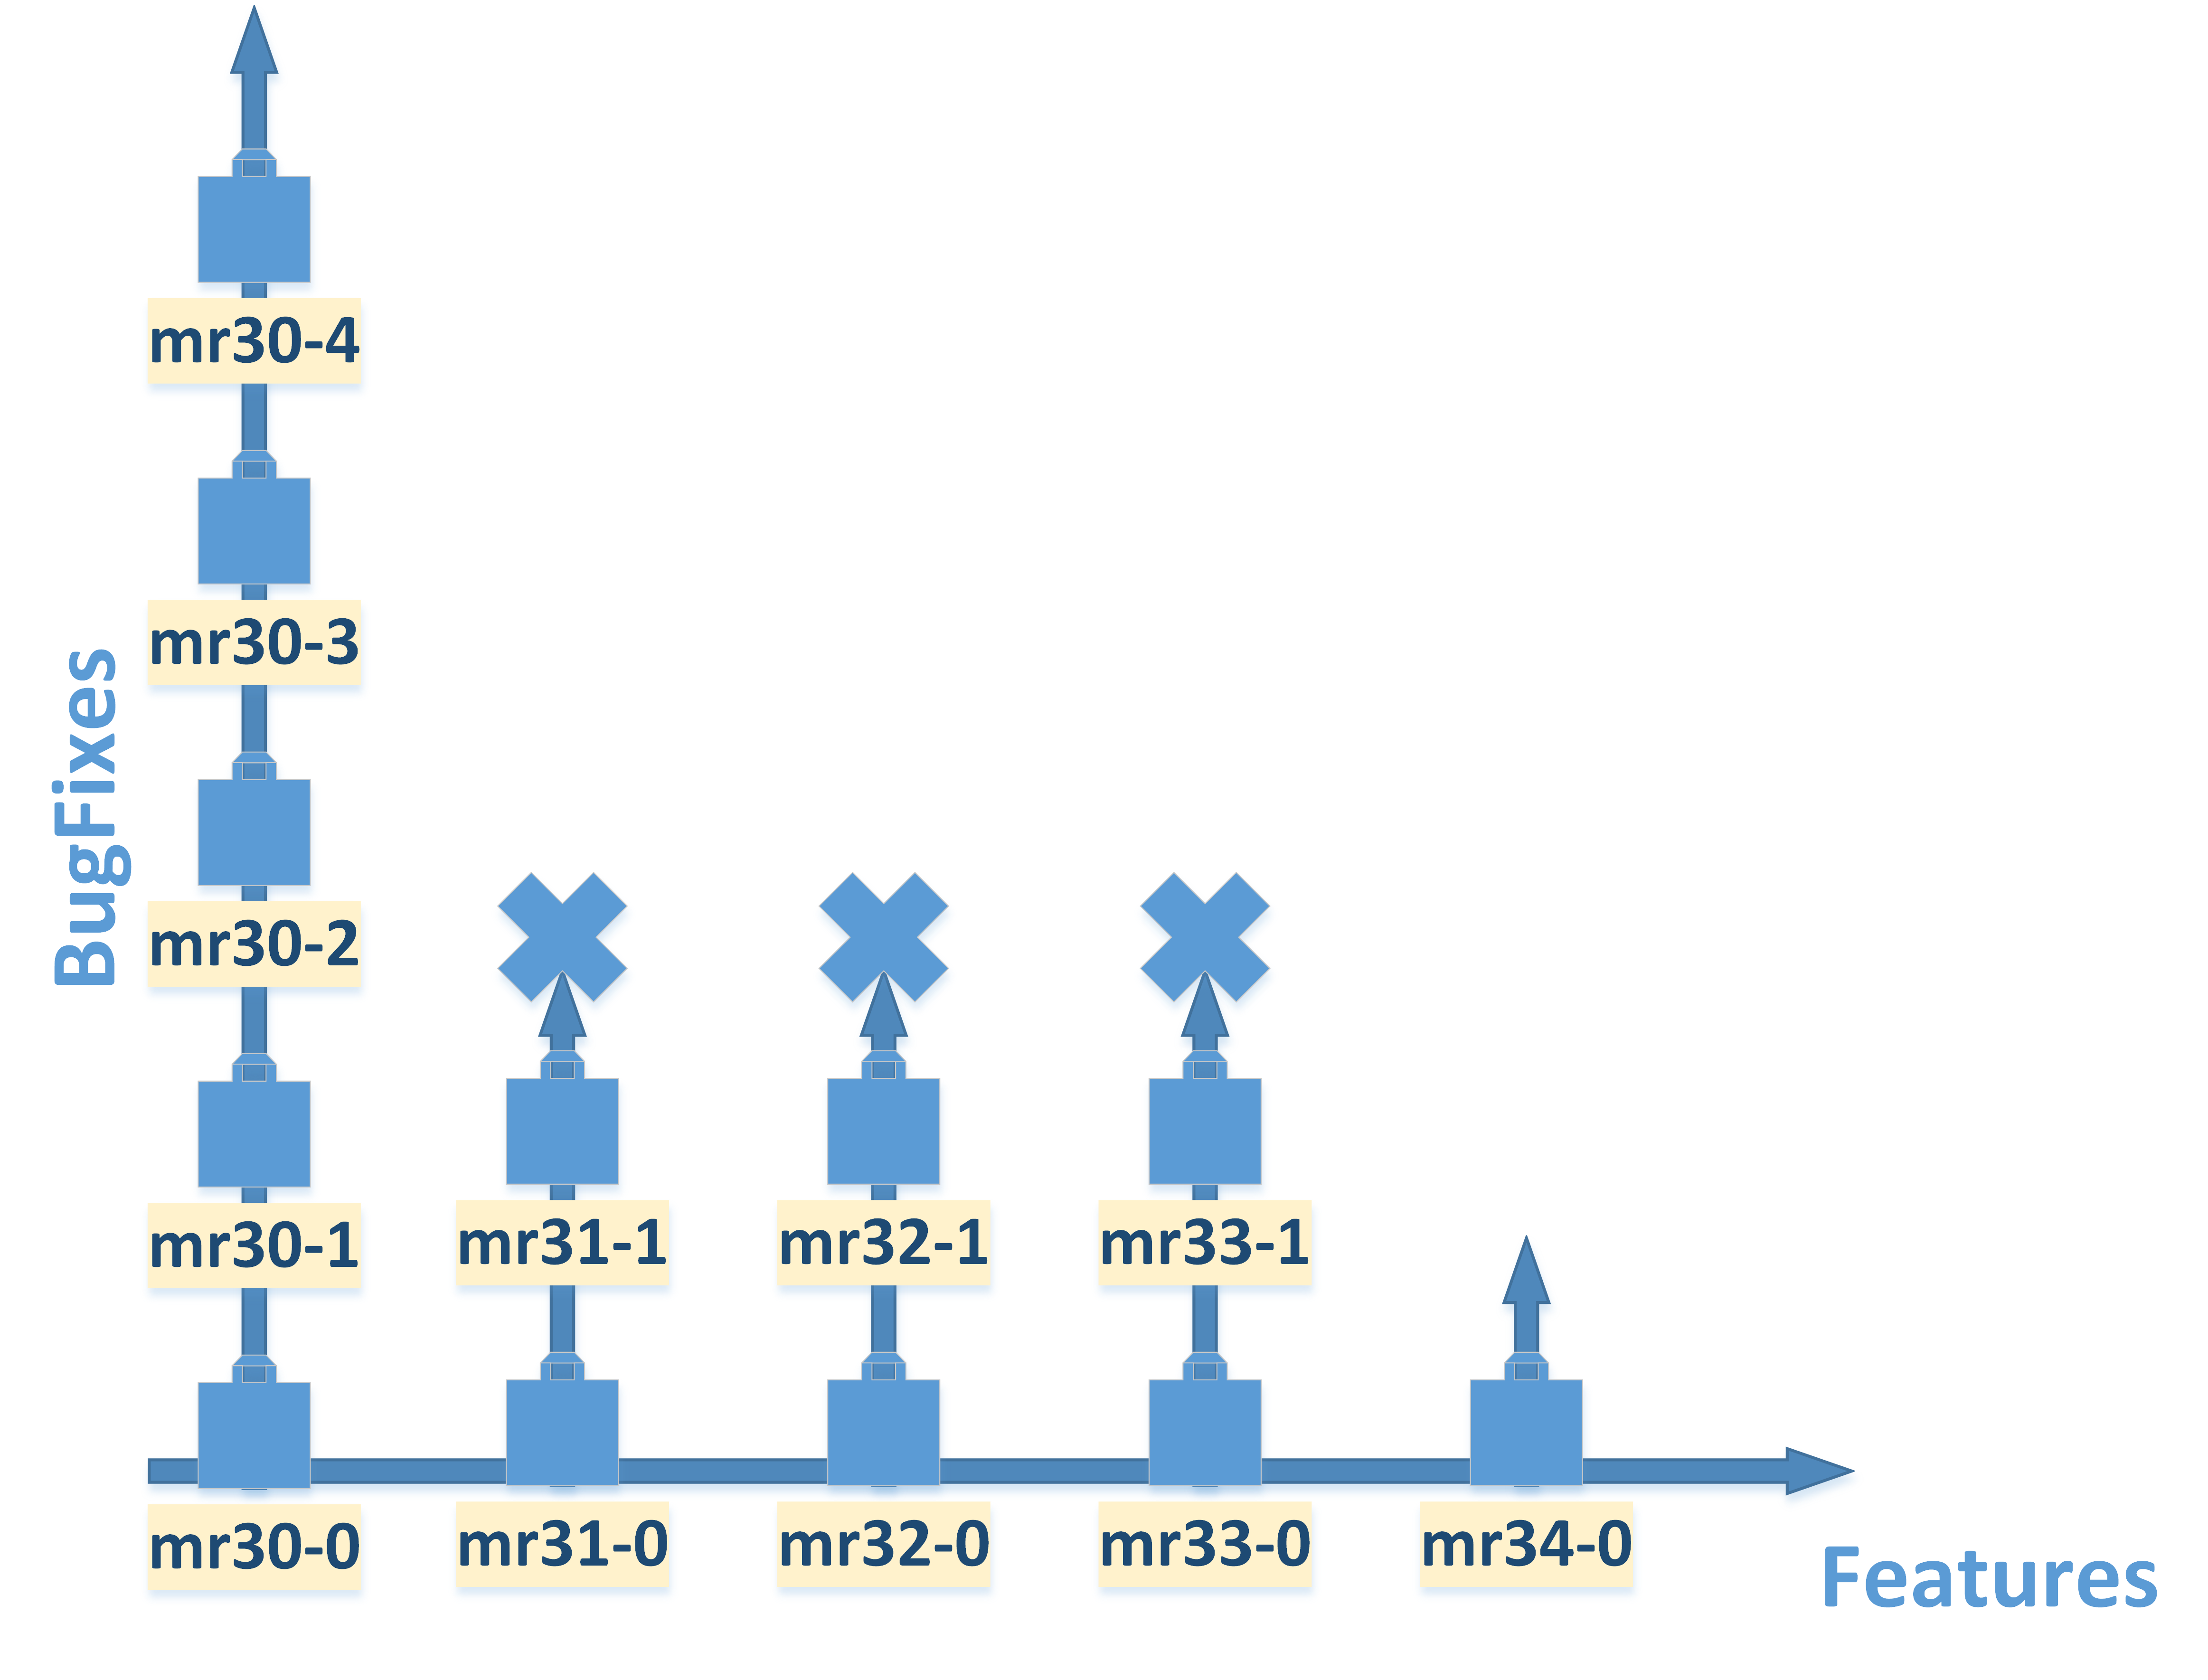
\includegraphics[width=10cm]{05_releases_graph_report.png}
\end{figure}

Данный подход позволяет:

\begin{enumerate}
  \item дать стабильность в LTS релизах;
  \item держать высокий темп выхода новых версий для заказчиков;
  \item продолжать заниматься разработкой, а не ожидать фидбэка/багрепортов;
  \item стабилизировать новые версии по мере получения фидбэка/багрепортов.
\end{enumerate}

\subsection*{Цикл разработки}

Заказчики хотят получать оплаченные новые возможности точно в срок.
На первый взгляд опыт разработки показывает, что это невозможно. Но это не так. Любые даже самые большие задачи могут быть разбиты на мелкие подзадачи, время на разработку которых возможно подсчитать. При относительно большом цикле (спринте), количество мелких задач, которые могут быть выполнены за определенный срок, стабильно. Не все задачи будут выполнены, но при правильном подсчете этот процент будет мал. В процессе фактической разработки может возникнуть определенное количество новых задач, они тоже должны быть заложены в план. Правильный подсчет времени и количества мелких задач, которые может выполнить отдел разработки в целом,  зависит от грамотности лидеров групп (team lead).

Был предложен следующий цикл разработки:

\begin{figure}[h!]
  \centering
  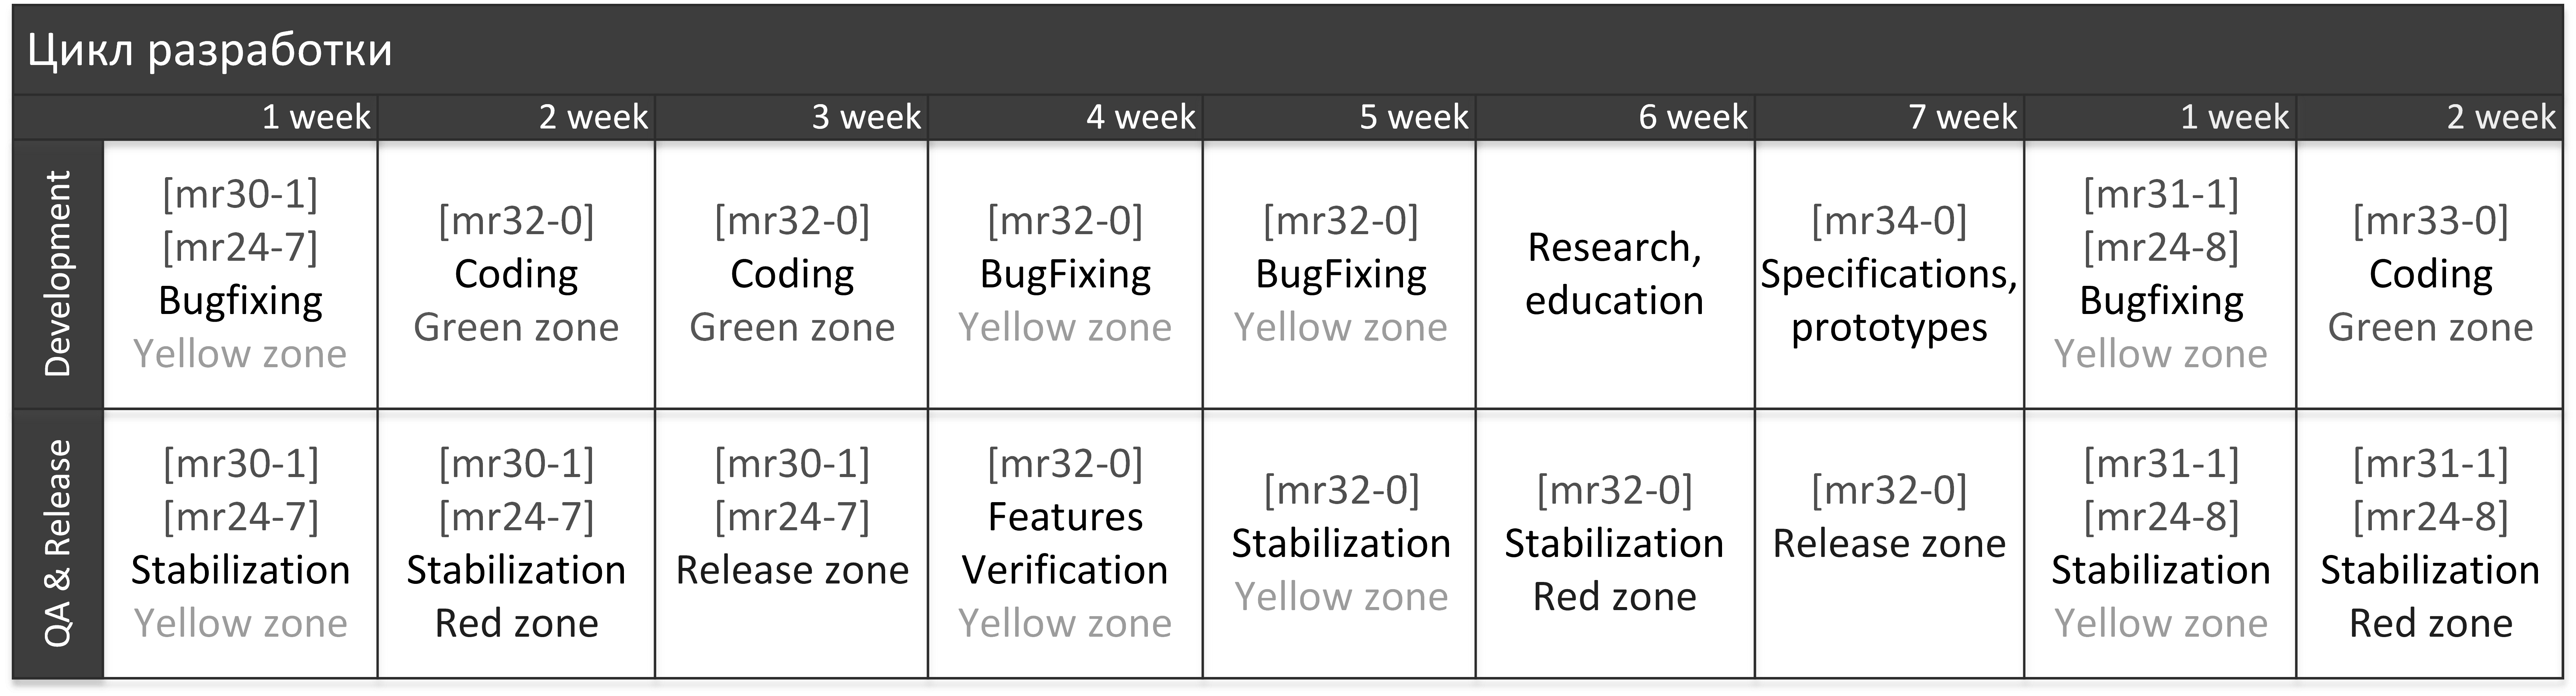
\includegraphics[width=11cm]{05_circle_v3.png}
\end{figure}

\subsection*{Создание спецификаций}

Невозможно гарантировать разработку новых возможностей вовремя, если конечному разработчику не понятны требования заказчика. Потому никакие запросы на новые возможности не будут приняты от заказчика (и не будут названы сроки) пока не будет создана исчерпывающая спецификация, которую примет и заказчик и лидеры групп в отделе разработки. Спецификация должна быть полностью понятна лидерам групп, которые разобьют ее на подзадачи и подсчитают сколько нужно времени на реализацию каждой из них, только после этого заказчику будут названы сроки.

\subsection*{Быстрое развертывание среды разработки}

Используются OpenSource"=решения Jenkins, VirtualBox, Vagrant.

Каждому разработчику, что бы начать исправлять ошибку или писать код, нужно иметь личную систему с установленной копией продукта который он разрабатывает. В больших и сложных продуктах довольно долго подготавливать правильно установленный и настроенный продукт (например, базу данных Oracle), это может длиться от нескольких часов до нескольких суток. При высоком темпе выпуска новых версий эта проблема многократно усиливается. Чтобы ускорить процесс развертывания среды разработки был полностью автоматизирован процесс создания образов виртуальных машин для всех версий продукта, для всех платформ с помощью Jenkins CI. Эти образы используются в самом Jenkins для запуска тестов во всех поддерживаемых версиях продукта на всех возможных платформах. С помощью vagrant, гигабитной офисной сети и SSD разработчики могут разворачивать за считанные десятки секунд полностью готовую среду разработки из образа, который имеет актуальный код на нужной платформе.

\subsection*{Автоматизация тестирования}

Используемые OpenSource решения "--- Jenkins.
Код покрыт следующими видами тестов:

\begin{itemize}
  \item Unit test
  \item Functionality test
  \item Performance test
  \item Syntax test
  \item Style test
  \item Code analysis
  \item Compile test
  \item Memory leak test (valgrind)
\end{itemize}

\subsection*{Стабильный транк}

Используемые OpenSource решения "--- Git, Gerrit, gerrit"=tools,\linebreak Jenkins CI.

~

~

\begin{figure}[b]
  \centering
  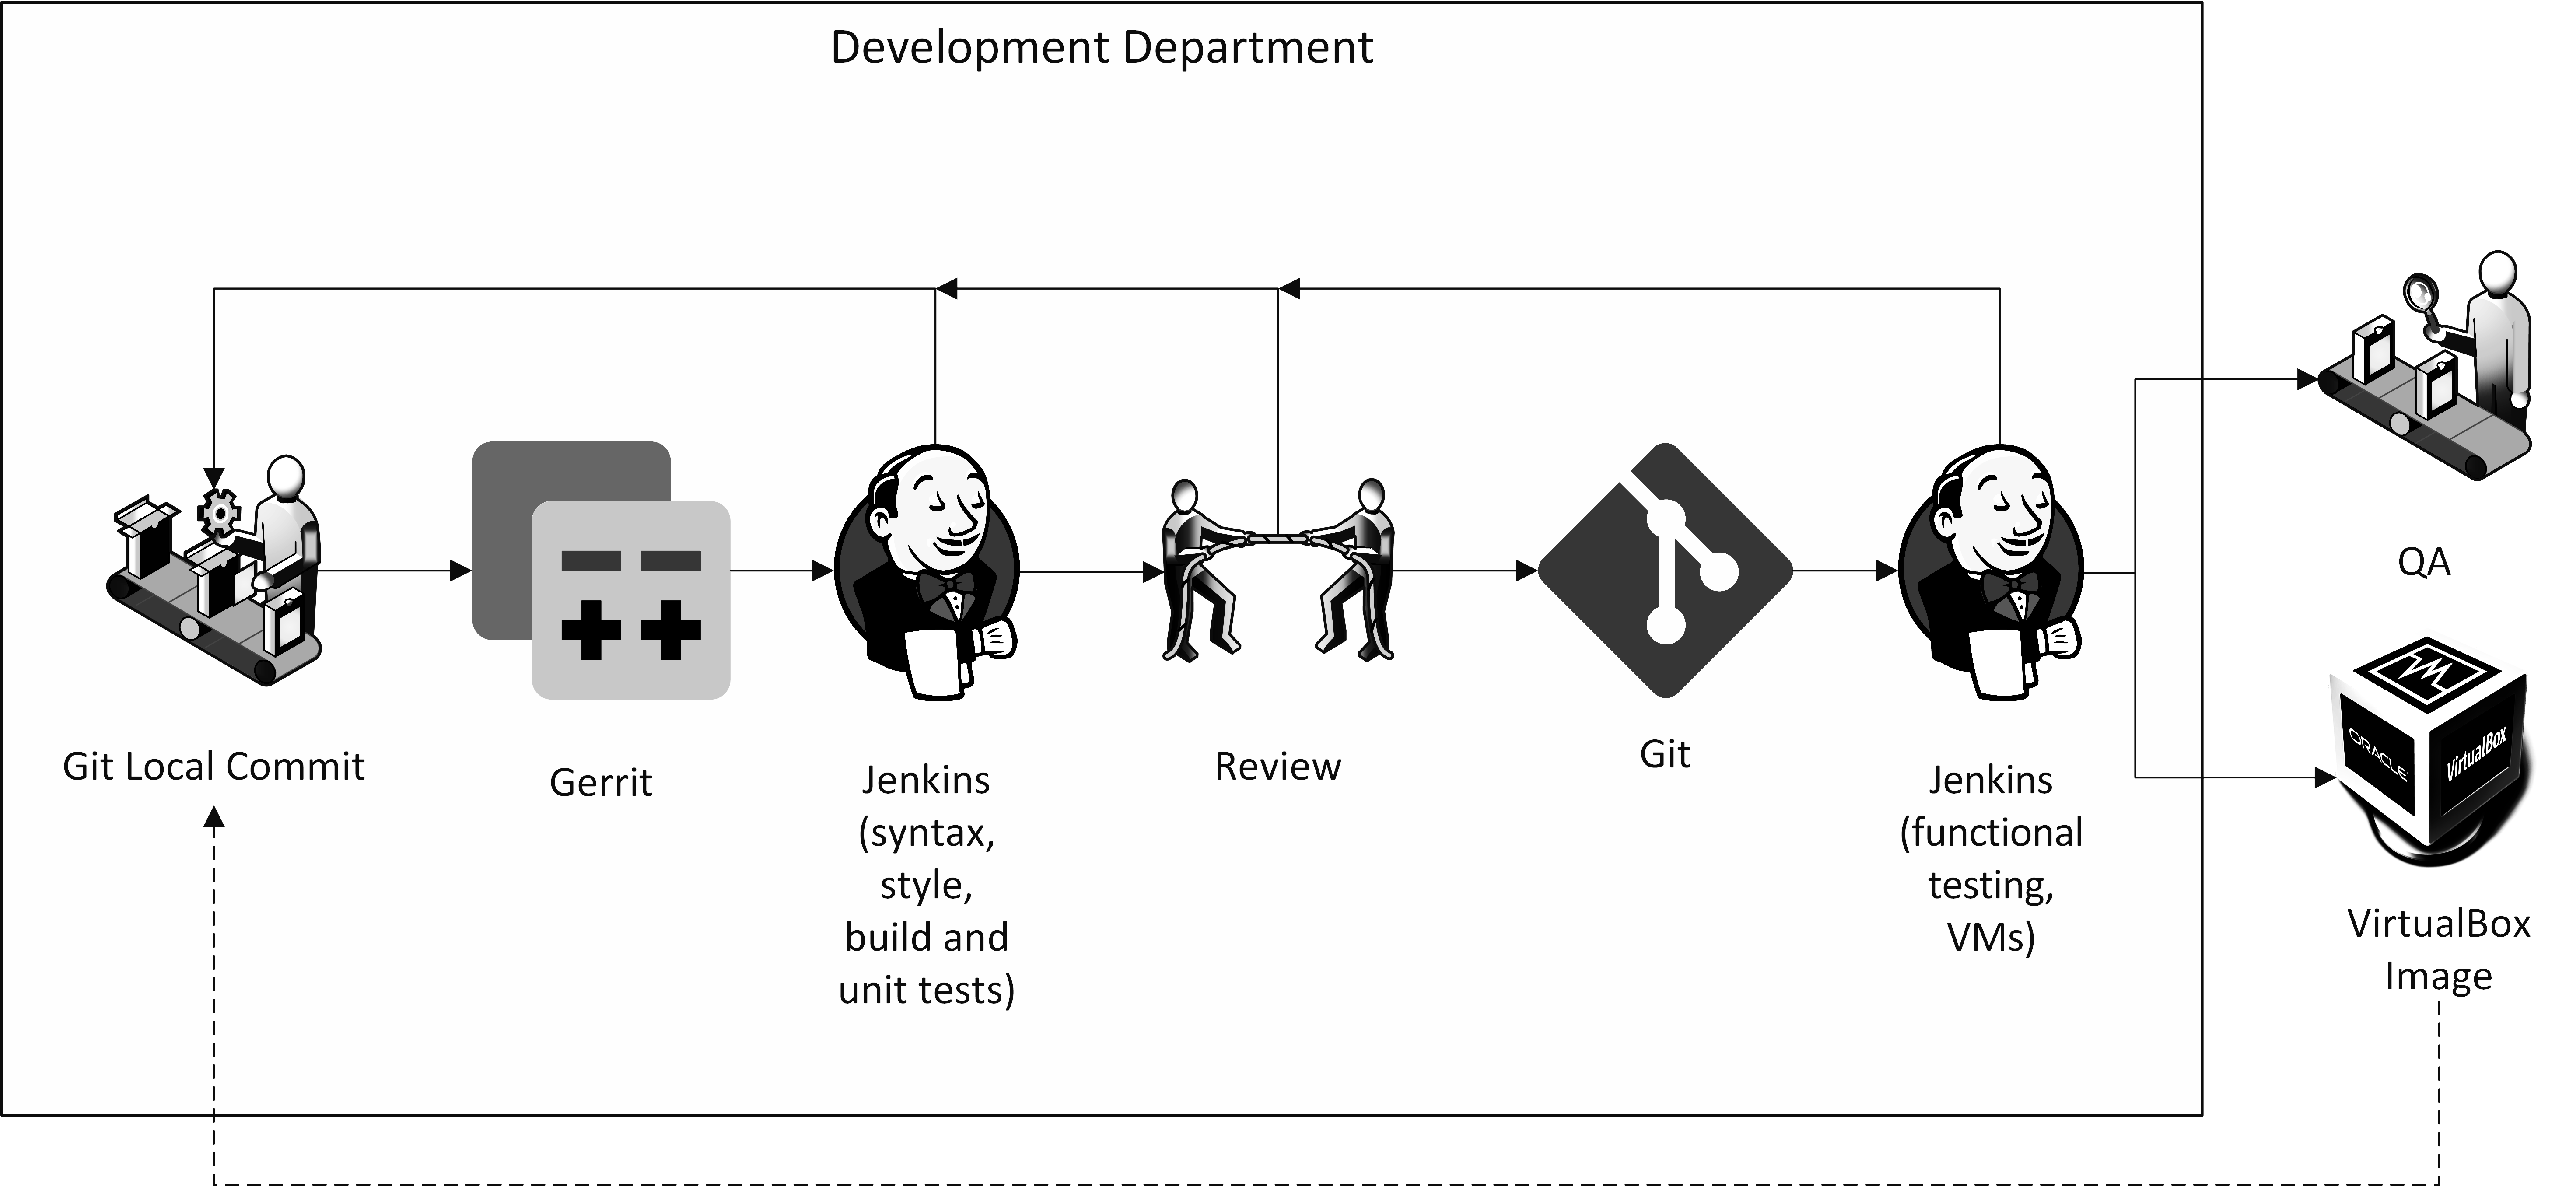
\includegraphics[width=11cm]{05_review.png} 
\end{figure}

Чтобы улучшить стабильность кода, был предложен следующий подход:

\begin{itemize}
  \item разработчик делает фиксацию изменений (коммит) в локальном git репозитории и запускает команду <<git review>>, которая отправляет изменения в gerrit;
  \item Gerrit задерживает изменения, не давая их отправить в центральный репозиторий до тех пор пока изменения не будут проверены рецензентами и автоматическими тестами в Jenkins;
  \item Gerrit запускает в Jenkins тесты, результат которых выставляется в виде положительной или негативной оценки;
  \item рецензенты могут комментировать код и выставлять оценки от $-2$ до $+2$. Код, который не имеет оценки $+2$ или имеет оценку $-2$, не может попасть в центральный репозиторий;
  \item когда рецензенты и Jenkins выставили положительные оценки, появляется кнопка <<Submit>> с помощью которой можно пропустить изменения в центральный репозиторий;
  \item раз в день запускаются тяжелые функциональные тесты, которые могут длиться всю ночь;
  \item на основе кода формируются образы виртуальных машин, которые с утра будут загружены разработчиками и QA.
\end{itemize}

\subsection*{Выводы}

Предложенные организационные изменения были проведены в компании PortaOne, Inc. на команде разработчиков из 50 человек и позволили разработчикам больше заниматься любимым делом и выдавать на 30\% больше кода. Отношения с клиентами улучшились благодаря выходу точно в срок новых версий продукта с заказанными функциональными возможностями. Стабильность кода увеличилась за счет введения процедуры review и автоматизации тестирования.


\end{document}




